\Subhead{1.3.1}{Воздействие гармонического сигнала. Синхронизация и захватывание колебаний}
Свободный автогенератор имеет устойчивую амплитуду $A_0$ и частоту $\omega_g$, но произвольную фазу. Слабый внешний сигнал прежде всего управляет этой фазой. \emph{Захватывание} означает общую частоту с постоянной разностью фаз; вне захвата возможно затягивание частоты и биения.

Для конкретности добавим $f_s\cos\Omega t$ справа в \eqref{eq:vdp}, где $f_s$ --- сила на единицу массы. Выберем $x=A(t)\cos[\Omega t+\theta(t)-\pi/2]$, расстройку $\Delta=\omega_g-\Omega$. Усреднение даёт в первом резонансном приближении
\begin{equation}\label{eq:forcedSL}
 \dot A=\mu A(1-A^2/4a^2)+F\cos\theta,\qquad
 \dot\theta=\Delta-\frac F A\sin\theta,\quad F=\frac{f_s}{2\Omega}.
\end{equation}
$[F]=[A]/{\rm с}$: делить исходную силу на амплитуду без множителя $2\Omega$ нельзя. Если $F/A_0$, $|\Delta|\ll2\mu$, амплитуда восстанавливается быстрее фазы и $A\simeq A_0=2a$. Получаем уравнение Адлера
\begin{equation}\label{eq:adler}
 \dot\theta=\Delta-K\sin\theta,\qquad K=F/A_0.
\end{equation}
Захват существует при $|\Delta|\leq K$; внутри полосы устойчив корень $\sin\theta_*=\Delta/K$ с $\cos\theta_*>0$, поскольку $\delta\dot\theta=-K\cos\theta_*\delta\theta$. Полная ширина полосы равна $2K$. У её края восстановление фазы замедляется.

Вне полосы фаза проскальзывает. Время полного оборота и средняя частота биений:
\begin{equation}
 T_{\rm б}=\int_0^{2\pi}\frac{\dd\theta}{|\Delta-K\sin\theta|}
 =\frac{2\pi}{\sqrt{\Delta^2-K^2}},\qquad
 \Omega_{\rm б}=\sqrt{\Delta^2-K^2}.
\end{equation}
Средняя частота генератора $\Omega+\operatorname{sgn}(\Delta)\Omega_{\rm б}$ ближе к сигналу, чем $\omega_g$: это затягивание. При приближении к краю захвата биения замедляются до нуля. На осциллографе с синхронизацией от внешнего сигнала изображение генератора при захвате неподвижно, а вне захвата относительная фаза плывёт. При сложении сигналов видна огибающая биений.
\begin{center}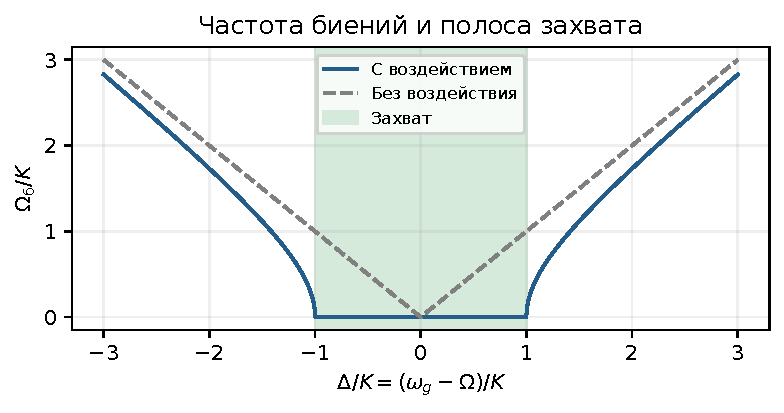
\includegraphics[width=.75\linewidth]{figures/locking.pdf}\end{center}
Результат относится к слабому воздействию и почти изохронной модели. Амплитудная зависимость частоты, шум и сильная связь меняют границы; фазовое уравнение не описывает все режимы исходного генератора.
